\chapter{Motor}
Bei der Auswahl und Integration eines Motors sind mehrere wichtige Fragen zu berücksichtigen, um eine optimale Leistung und Kompatibilität sicherzustellen.
Im Folgenden werden diese Fragen detailliert behandelt, wobei besonderes Augenmerk auf die Auswahl des Motors, seine Abmessungen, die Passform am Fahrrad, die Leistung in Watt und die ideale Positionierung des Motors gelegt wird.
\section{Arten von Fahrradmotoren}
%Welche Arten von Motoren gibt es?
E-Bikes verwenden drei Hauptarten von Motoren.
Der Mittelmotor befindet sich im Bereich des Tretlagers und bietet eine ausgeglichene Gewichtsverteilung, ein natürlicheres Fahrgefühl und eine effiziente Kraftübertragung durch die Mitte des Rahmens.
Im Gegensatz dazu ist der Hecknabenmotor im Hinterrad integriert und ermöglicht eine einfache Installation, kann jedoch das zusätzliche Gewicht die Fahrstabilität beeinträchtigen.
Der Frontnabenmotor befindet sich im Vorderrad und bietet ebenfalls eine einfache Installation, aber ein erhöhtes Lenkerdrehmoment kann das Lenkverhalten beeinflussen.
Die Wahl des Motors hängt von den individuellen Vorlieben des Fahrers und den Fahranforderungen ab.
\begin{figure}[h]
    \centering
    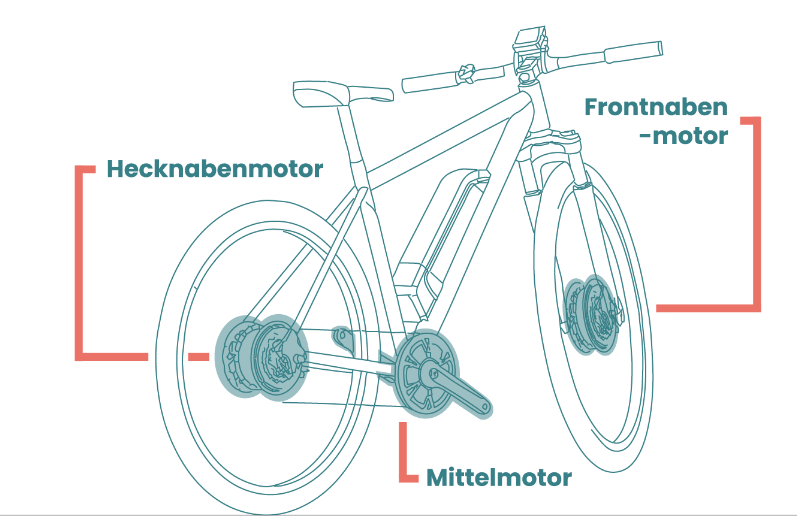
\includegraphics[width=10cm]{images/Motor_Arten}
    \caption{Motorenarten\cite{noauthor_e-bike_nodate}}%
    \label{fig:7}
\end{figure}
%Mittelmotor

\subsubsection*{Mittelmotor}
Ein Mittelmotor bei einem E-Bike befindet sich im Bereich des Tretlagers, also dort, wo üblicherweise auch die Kurbelgarnitur sitzt.
Im Gegensatz zu einem Heckmotor, der sich im Hinterrad befindet, oder einem Frontmotor, der sich im Vorderrad befindet, bietet ein Mittelmotor einige Vorteile:\\

Der Mittelmotor zeichnet sich durch eine ausgeglichenere Gewichtsverteilung aus, da er sich im Bereich des Tretlagers befindet.
Dadurch befindet sich der Schwerpunkt des Fahrrads näher am Boden, was zu einer besseren Fahrstabilität führt.
Dieses Merkmal ist besonders vorteilhaft beim Fahren auf unebenem Gelände oder in Kurven.
Zudem bietet der Mittelmotor ein natürlicheres Fahrgefühl, da er das Treten ähnlich wie ein herkömmliches Fahrrad unterstützt.\\

Ein weiterer Vorteil des Mittelmotors liegt in seiner Effizienz.
Durch die direkte Übertragung der Kraft auf das Antriebsritzel kann der Motor den Gangwechsel des Fahrers besser nutzen.
Dadurch wird die verfügbare Energie effizienter genutzt, was zu einer längeren Reichweite pro Akkuladung führen kann.
Schließlich trägt die zentrale Position des Motors im Rahmen zu einer besseren Gewichtsverteilung bei.
Im Vergleich zu einem Heckmotor, der das Gewicht eher auf der hinteren Seite des Fahrrads platziert, hilft der Mittelmotor dabei, das Fahrrad weniger unausgewogen zu machen und eine angenehmere Fahrt zu ermöglichen.\\

Ein Nachteil des Mittelmotors ist, dass der Verschleiß an den Ritzeln und der Kassette höher sein kann als bei anderen Antriebssystemen.
Dies liegt daran, dass der Motor direkt auf das Antriebsritzel wirkt und somit eine erhöhte Belastung auf die Zahnräder ausübt.
Insbesondere bei intensiver Nutzung und häufigen Schaltvorgängen kann dies zu einem schnelleren Verschleiß führen.
Es ist daher ratsam, regelmäßige Wartung durchzuführen und verschlissene Teile rechtzeitig auszutauschen, um die Lebensdauer des Antriebssystems zu maximieren und eine optimale Leistung zu gewährleisten.\\

Die Funktionsweise des Mittelmotors besteht darin, dass er die durch das Treten erzeugte Kraft des Fahrers verstärkt, indem er sie durch das Antriebsritzel auf das Hinterrad überträgt.
Dies geschieht normalerweise über ein System aus Zahnrädern und einer Kette oder einem Riemen.
Der Motor wird von der Energie aus einem Akku gespeist, der am Fahrrad angebracht ist und über eine Steuerungselektronik mit dem Motor verbunden ist.
Diese Elektronik regelt unter anderem die Leistung des Motors und kann oft auch verschiedene Fahrmodi und Assistenzniveaus bieten.

%Bild von mittelmotor
\begin{figure}[h]
    \centering
    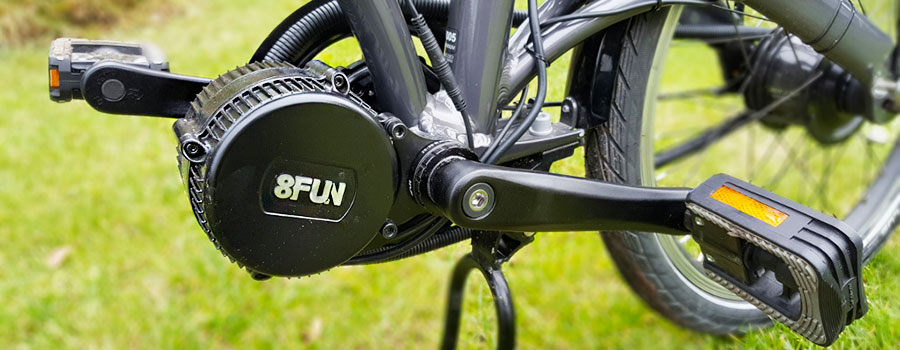
\includegraphics[width=10cm]{images/Mittelmotor-Fahrrad-nachruesten_F01.jpg}
    \caption{Mittelmotor\cite{noauthor_mittelmotor_nodate}}%
    \label{fig:8}
\end{figure}

\subsubsection*{Radnarbenmotor}
Der Nabenmotor ist in der Nabe des Hinterrads integriert und treibt dieses direkt an, wodurch die Kraftübertragung ohne Verluste direkt vom Motor auf das Laufrad erfolgt.
Ein Drehmomentsensor misst die Tretleistung des Fahrers und steuert die Motorunterstützung entsprechend.\\

Die Vorteile des Nabenmotors liegen im leisen Betrieb mit geringer Geräuschentwicklung, der Möglichkeit der Rekuperation zur Reichweitenerhöhung, der unauffälligen Integration in die Fahrradoptik und dem einfachen Einbau ohne spezielle Rahmenauslegung.\\

Jedoch weist der Nabenmotor auch einige Nachteile auf, wie eine ungünstige Gewichtsverteilung mit dem Schwerpunkt am Hinterrad, die Inkompatibilität mit Nabenschaltungen (nur Kettenschaltung möglich), die Tendenz zum Durchdrehen des Vorderrads bei Steigungen und Nässe, einen höheren Tretwiderstand durch das Getriebe im Hinterrad, problematischen Reifenwechsel durch integrierte Verkabelung und die Möglichkeit älterer Systeme, bei Dauerbelastung zu überhitzen.\\

Zusammengefasst bietet der Nabenmotor einen leisen Betrieb und Rekuperation, hat aber Nachteile bei der Gewichtsverteilung, Schaltübungskompatibilität und Lenkung, vor allem bei anspruchsvollem Gelände.\\

%Bild von Nabenmotor
\begin{figure}[h]
    \centering
    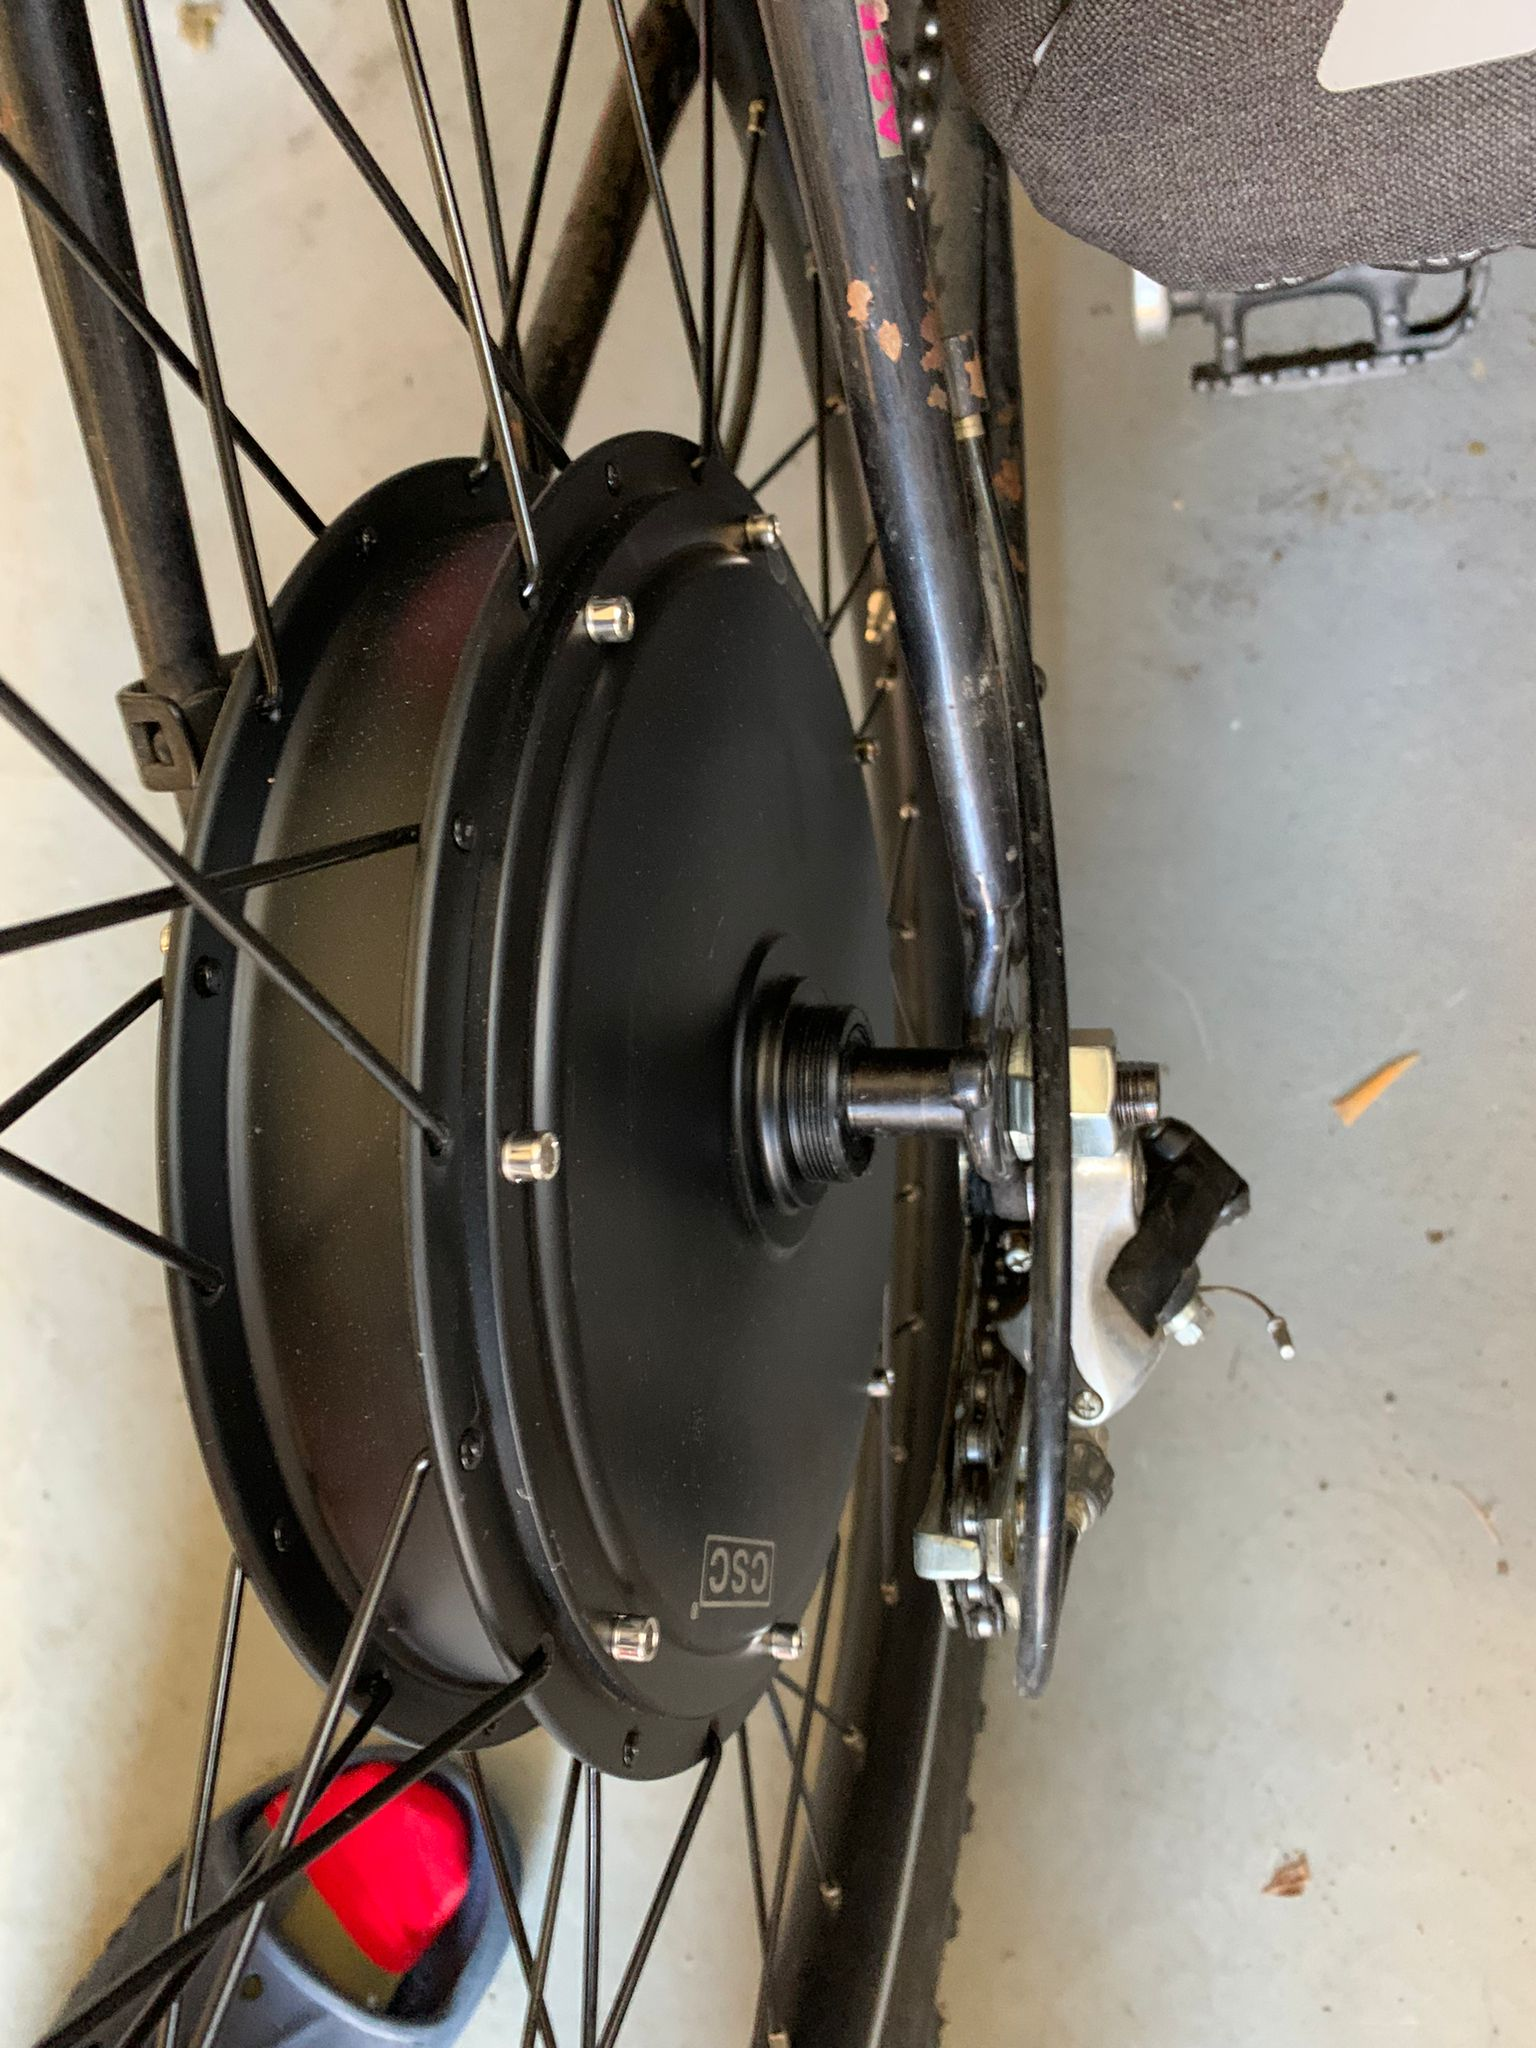
\includegraphics[width=10cm]{images/Radnabenmotor.jpg}
    \caption{Radnarbenmotor\cite{lorenz_scherrer_selbst_2023}}%
    \label{fig:9}
\end{figure}


Die Entscheidung für einen Nabenmotor basiert auf mehreren überzeugenden Argumenten.
Zunächst einmal ist die Installation eines Nabenmotors im Vergleich zu anderen Antriebssystemen, wie beispielsweise einem Mittelmotor, deutlich einfacher.
Da der Motor direkt in der Nabe des Rades integriert ist, erfordert seine Installation keine speziellen Rahmenanpassungen oder komplexe Montageprozesse.
Dies macht den Einbau sowohl für Hersteller als auch für Endbenutzer unkompliziert und kostengünstig.\\

Ein weiterer Vorteil des Nabenmotors liegt in seiner dezenteren Integration in das Design des Fahrrads.
Da der Motor im Inneren der Nabe verborgen ist, ist er für Außenstehende weniger sichtbar und beeinträchtigt nicht das ästhetische Erscheinungsbild des Fahrrads.
Diese unauffällige Integration kann besonders für Fahrer wichtig sein, die ein elegantes und minimalistisches Design bevorzugen.\\

Darüber hinaus weist der Nabenmotor tendenziell einen geringeren Verschleiß auf als andere Antriebssysteme.
Da die Kraftübertragung direkt vom Motor auf das Laufrad erfolgt, gibt es weniger bewegliche Teile und somit weniger Anfälligkeit für Verschleißerscheinungen.
Dies führt zu einer längeren Lebensdauer des Antriebssystems und reduzierten Wartungskosten für den Fahrer.\\

Schließlich bietet der Nabenmotor ein großes Potenzial für Leistung.
Durch die direkte Kraftübertragung auf das Laufrad und die Möglichkeit einem hohen Drehmoment entwicklung kann der Nabenmotor beeindruckende Leistungen erbringen, insbesondere im Hinblick auf Beschleunigung und Bewältigung von Steigungen.
Diese Leistungsstärke macht den Nabenmotor zu einer attraktiven Option für Fahrer, die hohe Leistung und Effizienz von ihrem E-Bike erwarten.\\

Insgesamt bietet der Nabenmotor eine Reihe von überzeugenden Vorteilen, darunter eine einfache Installation, dezente Integration, geringeren Verschleiß und beeindruckende Leistungsfähigkeit.
Diese Argumente machen ihn zu einer attraktiven Wahl für diejenigen, die nach einem zuverlässigen und leistungsstarken Antriebssystem für ihr E-Bike suchen.\\
\subsubsection*{Funktionsweise eines Bürstenlosen Gleichstrommotors}


Bei den Radnarbenmotoren handelt es sich um einen Bürstenlosen Gleichstrommotor.
Der Motor wandeln elektrische Energie in mechanische um.

%Konstruktion von einem Bürstenlosen
%Der Motor besteht aus einenm rotor stator
Bürstenlose Gleichstrommotoren (BLDC-Motoren) gehören zu den effizientesten und leistungsstärksten Antriebslösungen in der heutigen Industrie.
Sie bestehen aus einem Rotor und einem Stator, wobei der Stator die feststehende Komponente und der Rotor die sich drehende ist.
Links ist der Rotor zusehen und recht der Stator \ref{fig:11}

\begin{figure}[h]
    \centering
    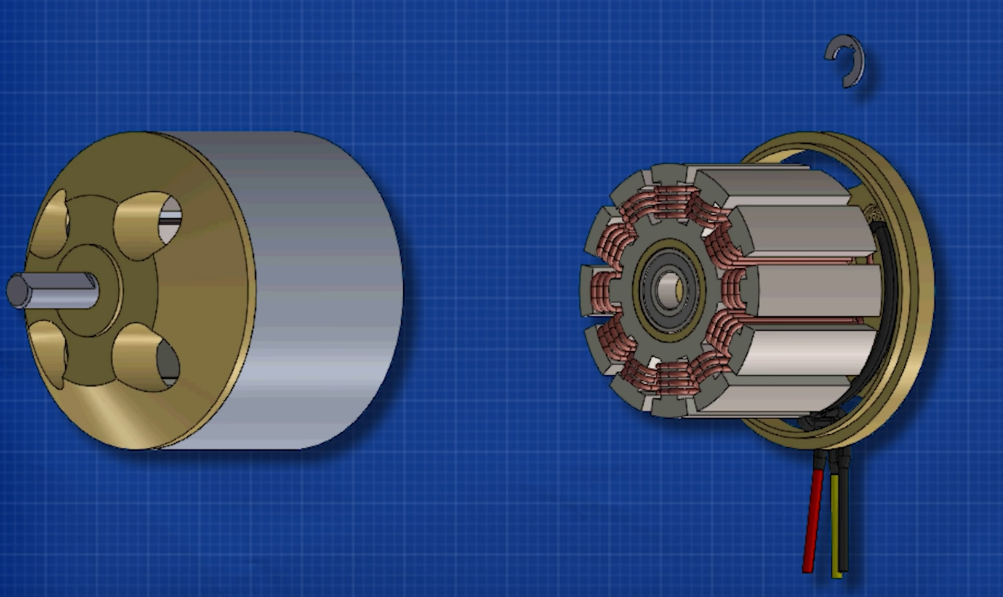
\includegraphics[width=10cm]{images/RotorStator.png}
    \caption{Rotor und Stator\cite{ingenieursmentalitat_burstenloser_2022}}%
    \label{fig:11}
\end{figure}

%Was bedeuteten Zähne des Stators?
Die Zähne des Stators sind die hervorstehenden Teile des Statorblechs, die dazu dienen, die Spulen zu umgeben und zu führen.
Sie sind strategisch angeordnet, um ein magnetisches Feld zu erzeugen, das den Rotor antreibt.  \ref{fig:11}\\

%Was machen die Spulen? und in welche Phasen gruppen sind sie aufgeteilt?
Die Spulen im Stator sind für die Erzeugung des magnetischen Feldes verantwortlich, das den Rotor antreibt.
Sie sind in drei Phasengruppen unterteilt: U, V und W. Diese Phasengruppen sind jeweils um 120 Grad versetzt, um ein gleichmäßiges Drehmoment zu erzeugen.\\

%Warum sind die benachbarten Spulen in verschiedene Richtungen gewickelt?
%Was bedeutet dlrk-Wicklung?
Die benachbarten Spulen sind in verschiedene Richtungen gewickelt, um sicherzustellen, dass sich das magnetische Feld gleichmäßig um den Rotor verteilt und somit ein reibungsloser Betrieb gewährleistet ist.
Diese Wickeltechnik wird auch als dlrk-Wicklung bezeichnet \ref{fig:12}.\\

\begin{figure}[h]
    \centering
    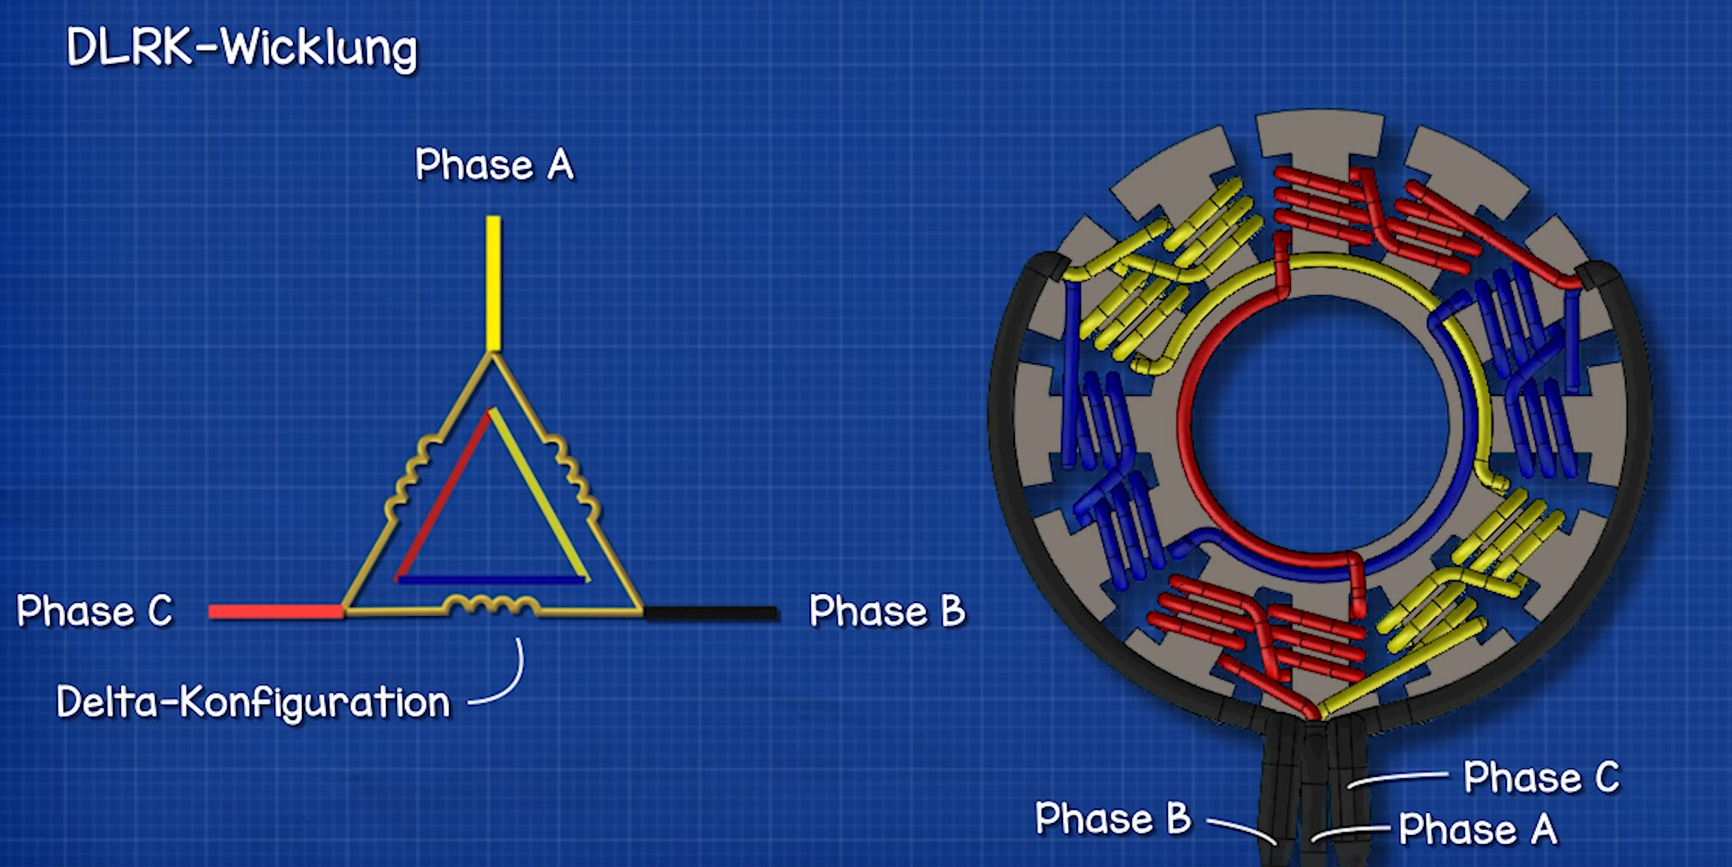
\includegraphics[width=10cm]{images/DLRK-Wicklung.png}
    \caption{DLRK-Wicklung\cite{ingenieursmentalitat_burstenloser_2022}}%
    \label{fig:12}
\end{figure}

%wue sind die permatnet magneten am Rotor angebracht?
Die Permanentmagnete am Rotor sind so angebracht, dass sie eine feste und starke magnetische Kraft erzeugen.
Sie sind in einer bestimmten Anordnung platziert, um ein optimales magnetisches Feld zu erzeugen und somit eine effiziente Drehbewegung zu ermöglichen.\\
%Wie sind sie anbracht?
%Die anzahl der Magneten und spulen unterscheiden sich damit sie sich nicht ausrichten
Die Anzahl der Magneten und Spulen kann variieren, um sicherzustellen, dass sich diese nicht ausrichten und somit das gewünschte Drehmoment erzeugt wird.
Durch diese Unterschiede in der Anordnung wird eine gleichmäßige und stabile Leistung des Motors gewährleistet.\\

%Funktionsweise


%Bild von Nabenmotor


%ein BLDC_Motor vs ein DC-Motor


\subsection{Energierückgewinnung}\label{subsec:energieruckgewinnung}

Radnabenmotoren bieten einen weiteren Vorteil: die Stromrückgewinnung.
Durch ihre Konstruktion ermöglichen sie es, kinetische Energie während des Bremsens in elektrische Energie umzuwandeln.
Dies geschieht, indem der Motor als Generator fungiert.\\

Der BLDC-Motor, der in Radnabenmotoren verwendet wird, kann seine Rolle ändern und als Generator arbeiten, wenn er dem Drehmoment entgegenwirkt.
Bei dieser Umkehrung des Betriebsmodus des Motors wird die mechanische Energie des rotierenden Rades in elektrische Energie umgewandelt, die dann in einer Batterie gespeichert oder direkt verwendet werden kann.
Diese Stromrückgewinnungsfunktion ist besonders nützlich in Anwendungen, in denen häufiges Bremsen oder Abbremsen erforderlich ist, wie zum Beispiel bei Elektrofahrrädern.
Sie trägt nicht nur zur Verbesserung der Energieeffizienz bei, sondern kann auch die Reichweite des Fahrzeugs erhöhen und die Lebensdauer der Bremsen verlängern, da weniger mechanische Bremsen verwendet werden müssen.
Zudem verbessert sie den Bremsweg des E-Bikes.
Hier ist zu sehen wie viel Strom bei sehr starken Abbremsen in die Batterie zurückfließt~\ref{fig:38}.
\begin{figure}[h]
    \centering
    \includegraphics[width=5cm]{images/ernergierück}
    \caption{Energierückgewinnung bei starken Abbremsen\cite{lorenz_scherrer_selbst_2023}}
    \label{fig:38}
\end{figure}

\subsection{Gleichstrombremsen Funktion}
Wenn der Stator an eine Gleichspannungsquelle angeschlossen wird, fließt ein Gleichstrom durch die Wicklung.
Dieser Gleichstrom erzeugt ein magnetisches Gleichfeld.
Dieses Gleichfeld induziert in dem darin rotierenden Läufer eine Spannung.
Durch den Kurzschluss der Läuferwicklung fließt in dieser ein Strom.
Aufgrund des geringen Widerstandes des Läufers genügen bereits kleine induzierte Spannungen, um im Läufer einen hohen Strom zu erzeugen.
Dieser Strom erzeugt im Rotor ein Magnetfeld.
Dieses Magnetfeld übt auf die stromdurchflossenen Leiter des Rotors eine Kraft aus, die nach der Lenz'schen Regel so gerichtet ist, dass der Rotor abgebremst wird[4], wodurch die Drehzahl des Motors sinkt.
Gleichzeitig mit der Drehzahlabnahme sinkt die Frequenz der im Rotor induzierten Spannung und damit auch der induktive Blindwiderstand des Rotors.
Dadurch überwiegt nun der ohmsche Widerstand des Rotors.
Durch den nun überwiegenden ohmschen Widerstand nimmt die Bremswirkung mit abnehmender Drehzahl zu.
Das Bremsmoment bei der Gleichstrom-Auslaufbremsung fällt erst kurz vor dem Stillstand stark ab und geht bei Stillstand des Läufers gegen Null.
Nach dem Stillstand kann im Gegensatz zur Gegenstrombremsung kein Anlaufen des Motors in Gegenrichtung erfolgen.
%Rekubarionsbremse
%Wirbelstrombremse
%Generator
%Dynanamo

%\href{https://www.portescap.com/de-DE/wissen/dokumente-und-zeichnungen/white-papers/nutzung-eines-gleichstromb%C3%BCrstenmotors-als-generator}

%Im Controller ist wahrscheinlich ein gleich Spannungsrichter der die Spannung und die Stromstärke wieder an die Batterie weitergibt


\section{Position des Motors}
%Vorderrad oder Hinterradantrieb?
Die Wahl zwischen einem Vorderrad- oder Hinterradmotor bei einem E-Bike hängt von verschiedenen Faktoren ab, die sowohl die Leistung als auch das Fahrverhalten des Fahrrads beeinflussen können.
Beginnen wir mit dem Vorderradmotor: Ein klarer Vorteil liegt in der schnellen Umsetzbarkeit des Umbaus.
Die Installation gestaltet sich vergleichsweise einfach, da der Motor direkt in die Nabe des Vorderrads integriert wird.
Dies ermöglicht eine rasche Anpassung von herkömmlichen Fahrrädern zu E-Bikes.\\

Jedoch weist der Vorderradmotor einige Nachteile auf.
Aufgrund der direkten Kraftübertragung auf das Vorderrad kommt es schnell zum Durchdrehen, insbesondere auf rutschigem Untergrund oder bei Steigungen.
Dies beeinträchtigt das Fahrverhalten und die Traktion des Vorderrads negativ.
Darüber hinaus ist die Gewichtsverteilung problematisch, da ein Großteil des zusätzlichen Gewichts durch den Motor vorne am Fahrrad konzentriert ist.
Dies kann zu einem ungleichmäßigen Fahrgefühl führen, insbesondere bei höheren Geschwindigkeiten oder in Kurven.\\

Um diese potenziellen Probleme zu untersuchen, wurden zwei Experimente durchgeführt.
Diese Experimente zielen darauf ab, das Durchdrehen des Vorderrads unter verschiedenen Bedingungen zu untersuchen und die Auswirkungen auf das Fahrverhalten zu bewerten.
Die Ergebnisse dieser Experimente liefern wertvolle Erkenntnisse für die Entscheidungsfindung bei der Wahl des Motors.\\

Auf der anderen Seite steht der Hinterradmotor, der seine eigenen Vor- und Nachteile bietet.
Einer der offensichtlichen Nachteile ist die komplexere Installation im Vergleich zum Vorderradmotor.
Da der Motor in die Nabe des Hinterrads integriert wird, erfordert die Installation möglicherweise spezielle Anpassungen des Rahmens und der Verkabelung.
Dies kann zu einem längeren Installationsprozess führen und zusätzliche Kosten verursachen.\\

Darüber hinaus kann der Hinterradmotor die Kompatibilität mit Nabenschaltungen einschränken, da die meisten Hinterradmotoren nur mit Kettenschaltungen kompatibel sind.
Dies kann die Auswahl an verfügbaren Schaltung- und Gangoptionen für den Fahrer begrenzen.
Zudem kann der Einbau des Motors zu einem höheren Tretwiderstand führen, da das Getriebe im Hinterrad zusätzlichen Widerstand erzeugen kann.\\

Trotz dieser Nachteile bietet der Hinterradmotor auch einige wichtige Vorteile.
Die Gewichtsverteilung ist oft besser ausgeglichen als beim Vorderradmotor, da sich der Motor im hinteren Teil des Fahrrads befindet.
Dies kann zu einem stabileren Fahrverhalten beitragen, insbesondere bei höheren Geschwindigkeiten oder in Kurven.
Darüber hinaus ermöglicht die Integration des Motors in das Hinterrad eine unauffälligere Optik, da der Motor weniger sichtbar ist und das ästhetische Erscheinungsbild des Fahrrads weniger beeinträchtigt wird.\\

Die Entscheidung für einen Hinterradmotor wurde letztendlich aufgrund dieser verschiedenen Faktoren und den Ergebnissen der zwei Experimente getroffen.
Trotz der komplexeren Installation bietet der Hinterradmotor eine bessere Gewichtsverteilung, eine stabilere Fahrdynamik und eine unauffälligere Optik, was ihn zu einer attraktiven Option für viele Fahrradfahrer macht.\\
%Vorteile und nachteile

\section{Leistung des Motors}

Die Entscheidung über die Motorleistung für den Bau eines E-Bikes ist ein wichtiger Schritt, der sorgfältige Überlegungen erfordert.
Dabei müssen mehrere Faktoren berücksichtigt werden, um die optimale Leistung zu bestimmen.\\

Zunächst ist es wichtig zu erwähnen, dass das E-Bike nicht in seiner vorgefertigten Form gekauft werden kann, was bedeutet, dass der Motor separat erworben werden muss.
Dies eröffnet verschiedene Möglichkeiten für den Erwerb und die Installation des Motors.
Eine Möglichkeit besteht darin, einen Motor zu kaufen, an dem bereits Speichen und Felge angebracht sind, während eine andere Möglichkeit darin besteht, nur den Motor zu erwerben und Speichen sowie Felge selbst anzubringen.
Beide Optionen haben ihre Vor- und Nachteile.\\

Beim selbstständigen Anbringen von Speichen und Felge ist die Entscheidungsfreiheit hinsichtlich des Motors flexibler.
Allerdings geht dies mit zusätzlichem Arbeitsaufwand einher und birgt das Risiko, dass die Zusammenstellung möglicherweise nicht in der Lage ist, die auf den Motor ausgeübte Kraft zu bewältigen.
Im Gegensatz dazu kann bei einem vollständigen Motor mit Speichen und Felge davon ausgegangen werden, dass die Zusammenstellung die Kraftauswirkung aushält.\\

Nachdem diese Kriterien definiert wurden, wurde eine Marktanalyse durchgeführt, um festzustellen, welche Optionen verfügbar sind.
Basierend auf den identifizierten Anforderungen und den verfügbaren Optionen wurde die Entscheidung getroffen, einen 1500 Watt-Motor zu verwenden.
Diese Leistungseinstellung ermöglicht eine angemessene Motorleistung für das E-Bike, ohne dabei die Strukturintegrität des Fahrzeugs zu gefährden.
Durch die Verwendung eines Motors mit dieser Leistung kann eine ausreichende Unterstützung für das E-Bike gewährleistet werden, während gleichzeitig potenzielle Schäden vermieden werden.\\


\section{Reichweite}

Ein Reichweitentest wurde mit dem E-Bike durchgeführt, um die maximale Reichweite zu bestimmen.
Dafür wurde eine Strecke von etwa 22 Kilometern festgelegt.
Die spezifischen Geschwindigkeiten und Streckenparameter, unter denen der Test durchgeführt wurde, sind in diesen Bildern zu sehen. 
Einmal die allgemeinen Streckenparameter siehe Abbildung~\ref{fig:33} und das Geschwindigkeitshistogramm~\ref{fig:34}.
Vor und nach der Testfahrt wurde der Ladezustand der Batterie abgelesen.
Beim Start lag die Batterie bei 97\% und nach der Tour bei 54\% Siehe Abbildung: \ref{fig:31} und \ref{fig:32}.
Das Ergebnis zeigte, dass 43\% der Batteriekapazität verbraucht wurden.\\

Bei einer Hochrechnung, die auf den Testergebnissen basiert, ergibt sich eine potenzielle Reichweite von ungefähr 40 Kilometern bei maximaler Geschwindigkeit ohne eigene Tretunterstützung.
Wenn der Fahrer tritt und je nach gewählter Unterstützungsstufe, kann die Reichweite pro Akkuladung wahrscheinlich zwischen 100 und 150 Kilometern variieren.

%eine weitere möglichkeit ist den strom aus der Batterie zu messen bei gewissen geschwindigkeiten







